\section{VLSI implementation}
\graphicspath{{sec2/images/}}
The purpose of this section is to present the implementation of the designed IIR filter, which in this case is an IIR filter with an accuracy of 10 bits and order of 1. In \autoref{fig:filter_generic} the filter interface is shown, where the parallelism $n_b$ is set to 10 and since the order of the filter is 1, the necessary coefficients are $a_0, a_1, b_0, b_1$.

\begin{figure}[h]
	\center
	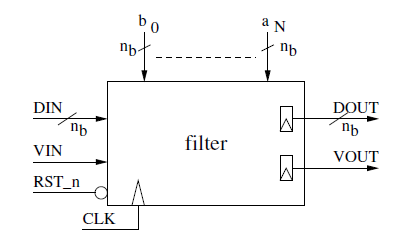
\includegraphics[width=0.4\textwidth]{filtro_generic.png}
	\caption{Filter pinout}
	\label{fig:filter_generic}
\end{figure}

\subsection{VHDL model}
At the input and output of the filter there are registers to synchronize the data with the clock and two validation signals for the data, $VIN$ and $VOUT$. In \autoref{fig:IIR_1} is shown the filter architecture, where the input and output registers have been neglected, the form used is the direct form II. The sampled input data enter from the $x[n]$ port, are processed and the results exit from the $y[n]$ port. The internal parallelism of the machine is different from the external one, to avoid the possibility of overflow with any combination of input data when summing, the precision has been extended to 12 bits by extending the sign to all input signals. The multiplier, on the other hand, has no problems of parallelism because it is possible to have sufficient precision by truncating the less significant bits at each multiplication and therefore having the same parallelism between input and output data. The internal register of the machine has an enable signal which is managed by the input data validation signal so that when invalid data is received, it does not sample keeping the correct output data.

\begin{figure}[h]
	\center
	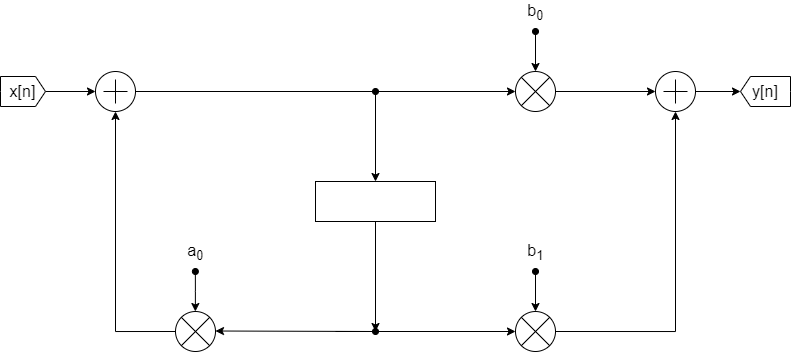
\includegraphics[width=0.8\textwidth]{iir_1.png}
	\caption{IIR filter architecture}
	\label{fig:IIR_1}
\end{figure}
\subsection{Simulation}
A solution with an input data generator and an output error checker has been adopted for the simulation of the circuit. A python script has been used to generate a sine waveform, which is processed in parallel by the designed circuit and the ideal model described in C. The output results are written on two files that are processed by an additional python script that computes the error as the difference between the output of the DUT and the C model.
In \autoref{fig:wave_start} is shown the wave with DUT signals. Note that when the $VIN$ signal becomes valid the circuit starts to sample the input data and after a latency of 2 clock periods the results are ready to output, so the $VOUT$ signal is asserted.

\begin{figure}[h]
	\center
	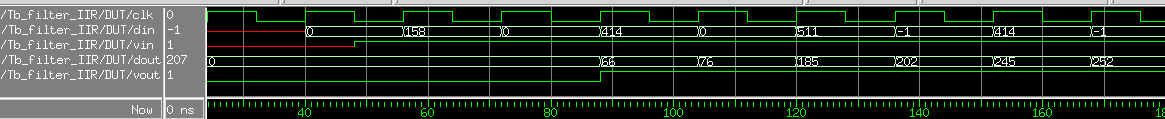
\includegraphics[width=1\textwidth]{wave_start.png}
	\caption{Start of the simulation}
	\label{fig:wave_start}
\end{figure}

In \autoref{fig:wave_vin} the correct functioning can be noticed even when $VIN$ is negated, in fact the data at the output of the filter, $d\_out$, remain unchanged when this situation occurs because the circuit stops sampling the input data. When $VIN$ returns to 1, after a latency of 1 clock period, the output data changes again.

\begin{figure}[h]
	\center
	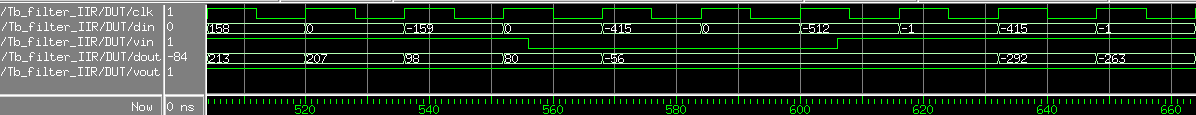
\includegraphics[width=1\textwidth]{wave_vin_0_1.png}
	\caption{Simulation of the $VIN$ signal transition}
	\label{fig:wave_vin}
\end{figure}

After verification of the correct timing of the circuit, the numerical results produced were checked. In \autoref{tab:tab_results} is shown an extract of the output data from the ideal model and the circuit designed with the same set of input data. It is noticeable that there is a perfect equality of results that confirms the correct operation of the designed filter.

\begin{table}[h]
\begin{center}
\begin{tabular}{|l|l|l|l|}
\hline
Input & DUT output & C model output & Error \\
\hline
511 & 252 & 252 & 0 \\
-1 & 213 & 252 & 0 \\
414 & 207 & 207 & 0 \\
-1 & 98 & 98 & 0 \\
158 & 80 & 80 & 0 \\
-1 & -56 & -56 & 0 \\
-159 & -77 & -77 & 0 \\
-1 & -188 & -188 & 0 \\
-415 & -206 & -206 & 0 \\
-1 & -250 & -250 & 0 \\
\hline
\end{tabular}
\end{center}
\caption{Results of the simulation}
\label{tab:tab_results}
\end{table}
\subsection{Logic Synthesis}
The synthesis of the circuit was done with the Synopsys software. The first objective is to determine the maximum frequency that will allow the correct operation of the circuit and its area. The standard port libraries provided have been used to automatically synthesize even the complex logical blocks such as adders and multipliers.
In a preliminary phase a clock with period $T_{clk} = \SI{10}{\nano\second} \pm \SI{0.07}{\nano\second}$ has been set. The result of the synthesis shows a slack of $+\SI{5.14}{\nano\second}$; the fact that the slack is positive implies that the clock constraints set have been met with the synthesis obtained.
To evaluate the maximum operating frequency of the circuit, a clock period of 0 has been set, so theoretically the negative slack obtained should correspond to the minimum necessary clock period. However, this is only partially true, since setting the clock period to the new value will still result in a negative slack. This behavior is due to the fact that the synthesizer changes the structure of the internal slack according to the constraint provided on the clock as you can see from the data on the area. It was necessary to iterate this procedure several times to obtain a slack equal to 0 and therefore the maximum operating frequency of the circuit. In \autoref{tab:timing_rep} a summary of the results obtained is shown.

\begin{table}[h]
\begin{center}
\begin{tabular}{|l|l|l|}
\hline
$T_{CLK}$ (ns) & slack (ns) & area $(\SI{}{\micro\meter})^2$ \\
\hline
10 & 5.14 & 1991 \\
0 & -3.13 & 2491 \\
4.10 & 0 & 2187 \\
16.4 & 11.54 & 1991 \\
\hline
\end{tabular}
\end{center}
\caption{Results of timing report}
\label{tab:timing_rep}
\end{table}

The second goal is to find area and power consumption by setting $T_{CLK} = 4 T_{min}$. For the area you can refer to \autoref{tab:timing_rep}. For the power computation, a record of the switching activity has been generated through a Modelsim simulation and saved on a vcd file, subsequently converted in saif file. The presence of these data serves during the calculation of the correct power consumption in the Synopsys environment. The results are shown in \autoref{fig:pow_rep_x4}.

\begin{figure}[htb!]
	\center
	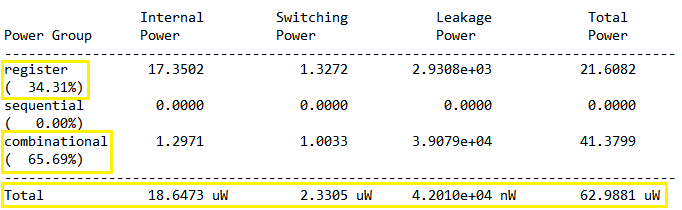
\includegraphics[width=0.8\textwidth]{rep_power_x4_mod.png}
	\caption{Power Report}
	\label{fig:pow_rep_x4}
\end{figure}

It can be seen that the power is divided between the registers and the combinatorial part with a preponderance of this second contribution, $65\%$, due to the presence of 3 multipliers and 2 adders in the designed architecture.

\subsection{Place \& Route}
The last operation is the place and route of the circuit using the Innovus software. The netlist generated by Synopsys with $T_{CLK} = 4 T_{min}$ and the standard libraries have been used as a starting point. After the various required steps the final circuit shown in \autoref{fig:layout} has been obtained.

\begin{figure}[htb]
	\center
	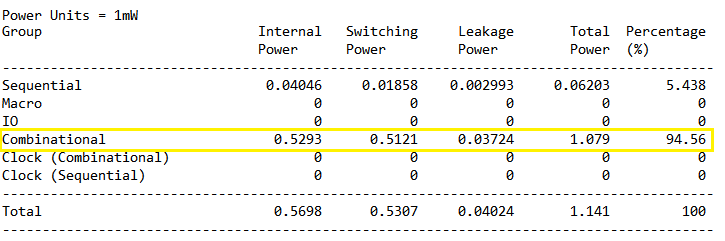
\includegraphics[width=0.7\textwidth]{rep_power_x4_cadence_mod.png}
	\caption{Post place \& route power report}
	\label{fig:cadence_pow_rep_x4}
\end{figure}

\begin{figure}[htb!]
	\center
	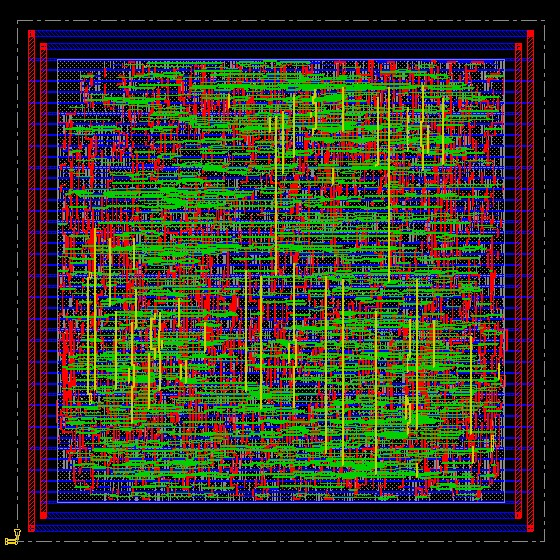
\includegraphics[width=0.5\textwidth]{IIR_filter_period_min_x4_place.jpg}
	\caption{Resulting layout}
	\label{fig:layout}
\end{figure}

The product layout has an area of $\SI{1959}{\micro\meter}^2$, which is in agreement with the estimated Synopsys' estimate shown in \autoref{tab:timing_rep}, with a total of 986 cells and 2455 gates. Then the timing analysis was launched to verify that the timing constraints were correct, then the connectivity and geometry was verified. Finally, using the switching activity calculated with Modelsim, the power consumption has been re-estimated. The results obtained are shown in \autoref{fig:cadence_pow_rep_x4}.


The power values obtained are in agreement with those obtained by Synopsys in \autoref{fig:pow_rep_x4}. Moreover, since the calculation at this level is much more accurate as it takes into account the physical layout of the circuit, it can be seen that in fact the consumption of the combinatorial part is prevalent.


\pagebreak
